
\documentclass[template=tabling,81pt,headonall]{azmoon}
\usepackage{xepersian}
\usepackage{amsfonts}
\usepackage{graphicx}
\graphicspath{ {./images/} }
\settextfont{Yas}
\setdigitfont{A Iranian Sans}
\usepackage{fontawesome5}

\printanswers
    \teacher{محمد صالح علی اکبری}
    \teachertitle{دبیر}
    \city{گناباد}
    \schooltitle{متوسطه دوره اول}
    \school{شاهد خاکپور}
    \grade{فرا پایه}
    \branch{-}
    \topic{ریاضی}
    \examdate{مهر 1402}
    \answertime{120 دقیقه}
    \begin{document}
	\begin{questions}
		\nointerlineskip%
		\vskip-\baselineskip
		\question{%
یک سال، ماه ژانویه درست چهار تا جمعه و چهار تا دوشنبه داشت، بیستم ژانویه آن سال چه روزی از هفته بوده است؟ ماه ژانویه ۳۱ روزه است.}\question{%
شکل زیر را به چهار تا شکل طوری تقسیم کنید که هر یک از آن‌ها مشابه شکل اصلی و ابعادش نصف آن باشد. \\ 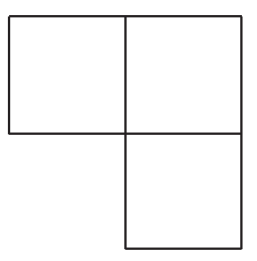
\includegraphics[scale = 0.2]{Screenshot from 2023-10-16 02-03-48}}\question{%
در صفحه‌ای یازده چرخ دنده به شکل زیر در یک زنجیره چیده شده‌اند. آیا ممکن ست که همه این چرخ دنده‌ها با هم بچرخند؟ \\ 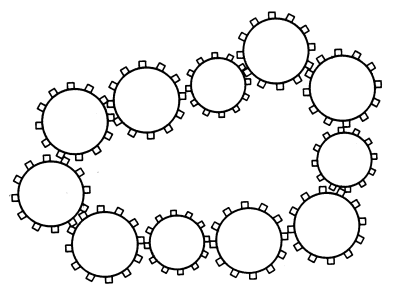
\includegraphics[scale = 0.15]{Screenshot from 2023-10-16 02-08-32}}\question{%
پنج قنجان مختلف و سه نعلبکی متفاوت در فروشگاه «مهمانی عصرانه» وجود دارد. به چند طریق می‌توان یک فنجان و یک نعلبکی خرید؟}\question{%
در فروشگاه «مهمانی عصرانه» چهار قاشق چایخوری مختلف هم وجود دارد. به چند طریق می‌توان یک سرویس چایخوری شامل یک فنجان، یک نعلبکی و یک قاشق خرید؟}\question{%
نقاط K , L, M, و N نقاط وسط اضلاع مستطیل ABCD و نقاط O, P, R و S نقاط وسط لوزی KLMN هستند. نسبت مساحت ناحیه‌های سایه خورده به مساحت مستطیل چند است؟ \\ 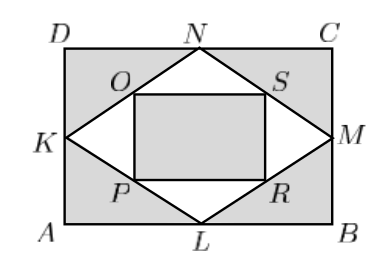
\includegraphics[scale = 0.3]{Screenshot from 2023-10-16 02-15-49} }\end{questions}
    \end{document}
    